\documentclass{article}

% Language setting Replace `english' with e.g. `spanish' to change the document
% language
\usepackage[english]{babel}

% Set page size and margins Replace `letterpaper' with `a4paper' for UK/EU
% standard size
\usepackage[letterpaper,top=2cm,bottom=2cm,left=3cm,right=3cm,marginparwidth=1.75cm]{geometry}

% Useful packages
\usepackage{amsmath}
\usepackage[pdftex]{graphicx}
\usepackage[colorlinks=true, allcolors=blue]{hyperref}
\usepackage{todonotes}
\usepackage{longtable}
\usepackage{booktabs}
\usepackage{multirow}
\usepackage{subcaption}
\usepackage{xcolor}
\usepackage{tabularray}
\usepackage{xspace} % For \xspace command
\usepackage{tikz}
\usetikzlibrary{shadings}
\usepackage{xifthen}

\newcommand{\colorbar}[6]% width,height,colors,label min,label max,label step
{   \begin{tikzpicture} \foreach \x [count=\c] in {#3}{ \xdef\numcolo{\c}}
    \pgfmathsetmacro{\piecewidth}{#1/(\numcolo-1)}
    \xdef\lowcolo{} \foreach \x [count=\c] in {#3} {   \ifthenelse{\c = 1} {} {
    \fill[left color=\lowcolo,right color=\x] ({(\c-2)*\piecewidth},0) rectangle
    ({(\c-1)*\piecewidth},#2); } \xdef\lowcolo{\x} } \draw (0,0) rectangle
    (#1,#2);
    \pgfmathsetmacro{\secondlabel}{#4+#6}
    \pgfmathsetmacro{\lastlabel}{#5+0.01}
    \pgfkeys{/pgf/number format/.cd,fixed,precision=2}
    \foreach \x in {#4,\secondlabel,...,\lastlabel} { \draw
    ({(\x-#4)/(#5-#4)*#1},0) -- ++ (0,-0.1) node[below=0.05,font=\tiny]
    {\pgfmathprintnumber{\x}}; }
    \end{tikzpicture}
}

\newcommand{\YC}[1]{\textcolor{red}{YC: #1}}

\newcommand{\0}{\mspace{9mu}} \newcommand{\navr}{$\nu_{\text{nav}}$\xspace}

\title{Numerical variability in structural MRI measurements on Parkinson's disease}

\author{Yohan Chatelain, Andrzej Sokołowski, Madeleine Sharp, Jean-Baptiste Poline, Tristan Glatard}

\begin{document}

\maketitle

\begin{abstract}
    Numerical variability, computational differences arising from floating-point
    arithmetic, poses a critical yet overlooked threat to reproducibility in
    clinical neuroimaging. We systematically quantify the impact of numerical
    variability in FreeSurfer, a widely-used MRI analysis tool, by analyzing how it
    processes identical brain scans under slightly different computational
    conditions—mimicking real-world variations across computers and software
    versions. To quantify this problem, we developed a metric that reveals when
    computational noise drowns out real biological signals. In Parkinson's disease
    patients, we found that up to half the measured brain differences could be
    computational artifacts rather than disease effects. This computational
    instability can flip research conclusions: the same data analyzed on different
    computers can yield opposite results about whether a brain region shows
    disease-related changes. When we applied our framework to landmark brain imaging
    studies, including ENIGMA consortium findings, many reported effects fell below
    the computational noise threshold, particularly in smaller studies. By
    quantifying and addressing numerical uncertainty, our study presents essential
    guidelines to enhance computational reliability and reproducibility in clinical
    neuroscience.
\end{abstract}

\section{Introduction}

Modern science is built on a foundation of computational analysis. From climate
modeling to genomics and neuroscience, complex software pipelines are
indispensable for transforming raw data into discovery. While researchers are
vigilant against software version changes and methodological errors, a more
fundamental challenge is often overlooked: the numerical variability of the
computations themselves. Seemingly deterministic algorithms can produce
slightly different results on each run due to factors like floating-point
arithmetic and parallelization, introducing a layer of computational
uncertainty that is rarely
quantified~\cite{botvinik2020variability,gronenschild2012effects,bhagwat2021understanding}.

This challenge is particularly acute in clinical research, where the goal is to
detect subtle biological signals of disease. In neuroimaging, for instance,
metrics such as cortical thickness are used as potential biomarkers to track
neurological disorders like Parkinson's disease
(PD)~\cite{haddad2023multisite}. If the computational noise in measuring these
biomarkers is on the same order of magnitude as the subtle brain changes caused
by the disease, any resulting scientific conclusions become inherently fragile.
This may contribute to the well-documented ``reproducibility crisis'' where
promising findings fail to translate into reliable clinical tools.

Here, we dissect the impact of within-software numerical variability on the
reliability of clinical neuroimaging research. We use Monte Carlo Arithmetic to
systematically assess FreeSurfer, a cornerstone software package, and develop a
novel framework—the Numerical-Anatomical Variability Ratio (\navr)—to directly
compare the magnitude of computational uncertainty to biological variability.
Using data from a major PD cohort, we (1) quantify how numerical instability
impacts group comparisons and brain-behavior correlations, (2) derive the
theoretical relationship between \navr and the reliability of statistical
effect sizes, and (3) apply this framework to re-evaluate the robustness of
landmark findings in the field.

\section{Impacts of numerical variability}

Numerical variability can have significant consequences for scientific
research, particularly in fields like neuroimaging where precise measurements
are crucial. In this section, we explore the various ways in which numerical
variability can impact research outcomes. We first demonstrate how numerical
instability can lead to fluctuating scientific conclusions. Next, we introduce
a framework to quantify the impact of numerical variability. Finally, we apply
this framework to re-evaluate landmark studies in the field, revealing
widespread potential for unreliable effect sizes.

\subsection{Numerical instability leads to fluctuating scientific conclusions}
% Comments
% - Extend the results section
% - First result on a page
%   - Writing for clinician audience with no expertise in computer science
%   - Writing for computer science audience with no expertise in neuroimaging  
% - Explain why MCA is important
% - Explain why figure significance_correlation_thickness is important
% - Explain why we choose Parkinson's disease MRI
%   - Explain the context of Parkinson's disease and its impact on neuroimaging research
%   - Cite Andrezj paper on Parkinson's disease MRI
%   - Use paper to replicate a representative of existing results and methodologie used for structural MRI analysis Parkinson's disease
% - refers to NARPS paper for the figures
% - Add more interpretation of the results
% - Get inspiration from the NARPS paper for the writing results section

Numerical instability is a pervasive issue in scientific computing,
particularly in neuroimaging, where complex algorithms process large datasets
to extract biologically relevant features.

The culprit is floating-point arithmetic—the way computers handle real numbers.
Just as 1÷3 cannot be perfectly represented in decimal (0.333\ldots), most
calculations produce tiny rounding errors. In a pipeline with millions of
calculations, these errors snowball into meaningful differences. Although the
IEEE-754 standard provides a consistent framework for representing and
manipulating floating-point numbers, their non-associativity leads to
variability in results when computations are performed in different
orders—determined by the underlying hardware and software forming a so-called
computational environment.

To measure this instability, we processed each brain scan 26 times while
introducing controlled computational perturbations—simulating the natural
variations that occur across different computers. We found that the numerical
variability significantly impacted the reproducibility of our findings. In many
cases, the same analysis performed on slightly different numerical states
produced divergent results, calling into question the reliability of the
original conclusions.

We assessed numerical variability in FreeSurfer 7.3.1 using Monte Carlo
Arithmetic (MCA)~\cite{parker1997monte} to simulate how will behave the
software under different execution environments (e.g. different hardware
configurations, operating systems, scientific computational libraries), more
particularly the Fuzzy-libm extension~\cite{salari2021accurate} that applies
random perturbations to mathematical library functions's output. MCA has
demonstrated its ability to simulate numerical variability in several
scientific domains, including
neuroimaging~\cite{kiar2020comparing,des2023reproducibility,chatelain2024numerical,vila2024impact}.
We executed 26 \texttt{recon-all} runs for each subject's MRI data from the
Parkinson's Progression Markers Initiative (PPMI), simulating 26 numerical
states.

For the same brain scans, statistical tests gave different answers depending on
computational conditions. A brain region showing 'significant' disease effects
in one run showed no effect in another—purely due to rounding errors.

We first tested the statistical significance of group differences between
Parkinson's disease (PD) patients and healthy controls (HC), and their
correlations with clinical measures (UPDRS scores), across the 26 MCA
repetitions. Similar to the NARPS study~\cite{botvinik2020variability} that
highlighted the impact of analytical variability in neuroimaging, we observed
substantial fluctuations in the results due to numerical variability. We used a
similar layout to NARPS paper to report the results, with the proportion of
statistically significant tests ($p < 0.05$) varied substantially for both
cortical thickness (Figure~\ref{fig:significance_correlation_thickness}) and
subcortical volumes
(Figure~\ref{fig:significance_correlation_subcortical_volume}). For many brain
regions, the significance of a finding was inconsistent, appearing in some
computational runs but not others. Ratios near 0.5 indicate maximal
uncertainty, where a reported result could be attributed to a lucky roll of the
computational dice. This variability in statistical significance suggests that
the conclusions drawn from these analyses are not robust and may be influenced
by the specific numerical state of the computation. This is specific to brain
regions, some regions showing high consistency across numerical states, while
others exhibit substantial variability. This instability is particularly
concerning when finding biomarkers for the Parkinson's disease progression, as
it suggests that the biological signals of interest may be obscured by
computational noise. Sokołowski et al.~\cite{sokolowski2024impact} highlighted
similar issues when playing with different FreeSurfer versions, showing that
the results can vary significantly between versions 5, 6 and 7. Biomarkers are
crucial for understanding disease mechanisms and tracking progression. Having
reliable biomarkers is essential to better understand the nature of the disease
which remains not well understood~\cite{bloem2021parkinson}.

This instability is also reflected in the effect sizes themselves. Partial
correlation coefficients and F-statistics from ANCOVA analyses showed
substantial spread around the unperturbed IEEE-754 results (red markers in
Figure~\ref{fig:statstest_coefficients_distribution} and
\ref{fig:navr_consistency_thickness}). This demonstrates that numerical
variability affects not only the binary outcome of statistical significance but
also the magnitude of the estimated effect, further complicating the
interpretation of results. We can notice that the unperturbed results (red
dots) are contained within the distribution of coefficients and F-statistics,
which indicates that our methodology is sound, but the variability in the
results highlights the need for caution in interpretation. In particular, when
interpreting results for possible clinical applications, it is important to
consider the potential impact of numerical variability on the robustness of
findings. Yellow dots around red ones can be seen as many potential results
that could be obtained by running the same analysis under computational
environments.

\begin{figure}
    \includegraphics[width=\linewidth]{figures/consistency/subcortical_volume_significance_correlation.pdf}
    \caption{ Proportion of significant tests ($p<0.05$) for subcortical volumes across 26 numerical perturbations.
        measures.\label{fig:significance_correlation_subcortical_volume}}
\end{figure}

\begin{figure}
    \centering
    \includegraphics[width=\linewidth]{figures/consistency/cortical_thickness_significance_correlation.pdf}
    \caption{Proportion of significant tests ($p<0.05$) for cortical thickness across 26 numerical perturbations.
        measures.\label{fig:significance_correlation_thickness}}
    \label{fig:navr_consistency_thickness_plot}
\end{figure}

\begin{figure}
    \includegraphics[width=\linewidth]{figures/consistency/subcortical_volume_coefficients_distribution.pdf}
    \caption{ Distribution of partial correlation coefficients (r-values) and
        F-statistics from ANCOVA across MCA repetitions for subcortical volume
        measures. Red dots represent the IEEE results. The top row shows
        r-values, while the bottom row shows F-values. The left column
        represents baseline analysis, and the right column represents
        longitudinal analysis.\label{fig:statstest_coefficients_distribution}}
\end{figure}

\begin{figure}
    \centering
    \begin{subfigure}[b]{\linewidth}
        \includegraphics[width=\linewidth]{figures/consistency/cortical_thickness_coefficients_distribution-Left.pdf}
        \caption{Left hemisphere}
        \label{fig:navr_consistency_thickness_left}
    \end{subfigure}

    \begin{subfigure}[b]{\linewidth}
        \includegraphics[width=\linewidth]{figures/consistency/cortical_thickness_coefficients_distribution-Right.pdf}
        \caption{Right hemisphere}
        \label{fig:navr_consistency_thickness_right}
    \end{subfigure}
    \caption{Distribution of partial correlation coefficients for cortical
        thickness across all subjects and regions. Red triangles indicate the
        IEEE-754 run for reference. The distribution shows the variability in
        the coefficients, with some regions exhibiting higher consistency than
        others. }
    \label{fig:navr_consistency_thickness}
\end{figure}

\subsection{A framework to quantify the impact of numerical variability}

% Comments:
% - Build a tool that can be broadly applied to any neuroimaging
% - Analytical modeling of sigma_d
% - Explain why having a tool is important
% - Why having a tool fast is important
%   - Measuring numerical variability is a time-consuming process
%   - Analytical modeling of sigma_d allows applying the tool to any neuroimaging papers, existing results.
% - Quality Control impact findings => a tool to find potentially unreliable results
% - To be general, we developped an analytical model
% - Refers to the online tool on yohanchatelain.github.io/brain-render

How much computational noise is too much? We developed the Numerical-Anatomical
Variability Ratio (\navr), a metric that answers this question by comparing
computational uncertainty to real biological differences between people. We
built this tool to be broadly applicable to any neuroimaging analysis, allowing
researchers to easily assess the impact of numerical variability on their
findings. Our metric works like a signal-to-noise ratio in reverse: when \navr
= 0.5, half the observed 'biological variation' is actually computational
noise. When \navr approaches 1, we're measuring noise, not brains. \navr is
defined as:
\[
    \nu_{\text{nav}} = \frac{\sigma_{\text{num}}}{\sigma_{\text{anat}}}
\]
where $\sigma_{\text{num}}$ is the numerical variability
(see~\ref{eq:sigma_num}) and $\sigma_{\text{anat}}$ is the anatomical
variability (see~\ref{eq:sigma_anat}).

Having a tool to quantify numerical variability is crucial for several reasons.
First, it allows researchers to assess the reliability of their findings and
reveal meaningful signals from noise. Second, it provides a framework for
comparing the impact of the numerical variability versus the anatomical
variability, enabling more informed decisions about study design and data
interpretation. Finally, it allows for the rapid assessment of numerical
variability in existing neuroimaging studies, facilitating the identification
of potentially unreliable results. Indeed, measuring numerical variability can
be a time-consuming process, especially when dealing with large datasets and
complex analyses. By providing an analytical model of \navr, we enable
researchers to apply this tool to any neuroimaging paper or existing results,
significantly speeding up the process of assessing numerical precision. We
developed an online
tool\footnote{\url{https://yohanchatelain.github.io/brain_render/}} that allows
researchers to threshold their results based on \navr values, providing a
practical way to identify potentially unreliable findings.

Figures~\ref{fig:navr_thickness} and \ref{fig:navr_subcortical} present the
\navr for cortical thickness and subcortical volumes. These brain maps
visualize the regions where the problem of numerical variability is most
severe. Regions with high \navr values (e.g., approaching 0.5, shown in warmer
colors) indicate areas where up to half of the observed variability is due to
computational noise rather than true anatomical differences, severely
compromising the ability to detect genuine biological effects.

We derived the theoretical relationship between \navr and the uncertainty in
Cohen's d, a standard measure of effect size:
\[
    \sigma_d = \frac{2}{\sqrt{N}} \text{\navr}
\]
where $\sigma_d$ is the standard deviation of Cohen's d and $N$ is the total
sample size. This formula provides a direct way to translate the numerical
stability of a measurement into its impact on statistical power and
reliability, offering a practical tool for researchers to gauge the robustness
of their findings.

\begin{figure}[h]
    \centering
    \begin{tikzpicture}
        \node[anchor=base,inner sep=10] at (0,0)
        {\includegraphics[width=\linewidth]{figures/NAVR_map/NAVR_subcortical_volume_all.png}\label{fig:navr_subcortical}};
    \end{tikzpicture}
    \subcaption{Subcortical volumes\label{fig:navr_subcortical}}
    \begin{tikzpicture}
        \node[anchor=base,inner sep=10] at (0,0)
        {\includegraphics[width=\linewidth]{figures/NAVR_map/NAVR_thickness_all.png}\label{fig:navr_thickness}};
    \end{tikzpicture}
    \subcaption{Cortical thickness\label{fig:navr_thickness}}
    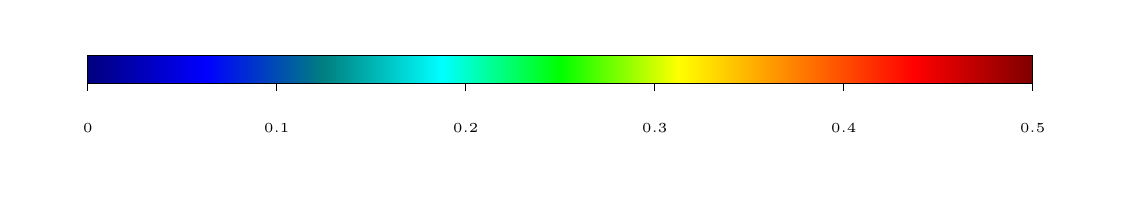
\begin{tikzpicture}
        \node[anchor=base,inner sep=10] at (0,0)
        {\colorbar{12}{0.35}{blue!50!black,blue,teal,cyan,green,yellow,orange,red,red!50!black}{0}{0.5}{0.1}};
    \end{tikzpicture}
    \caption{Numerical-Anatomical Variability Ratio (\navr) for subcortical volumes~\ref{fig:navr_subcortical} and cortical
        thickness~\ref{fig:navr_thickness} across regions and groups. Higher \navr values indicate
        greater computational uncertainty relative to biological variation. The
        color scale indicates the \navr value, with warmer colors indicating
        higher \navr values.}
\end{figure}

\subsection{Re-evaluating landmark studies reveals widespread potential for unreliable effect sizes}

The true test of our discovery: what happens when we apply this metric to the
field's most influential findings? ENIGMA~\cite{thompson2014enigma}—the world's
largest neuroimaging consortium—has shaped our understanding of psychiatric
disorders by analyzing tens of thousands of brain scans. When we applied our
computational noise threshold to their published brain maps, large regions went
black: the reported effects were smaller than measurement noise.

This finding raises important questions about the reliability of existing
neuroimaging literature. Are we overestimating the effects of certain brain
regions? Are there systematic biases in how we report and interpret these
findings?

Figures~\ref{fig:navr_enigma_thickness} and \ref{fig:navr_enigma_subcortical}
present the powerful results of this analysis. The left panels show the
original Cohen's d maps for various disorders, while the right panels show the
same maps after thresholding. Regions colored in black indicate where the
reported effect size is smaller than the underlying computational noise of the
measurement tool. While many of the core, highly significant findings of ENIGMA
remain robust (as expected from their large sample sizes), a considerable
number of secondary findings are shown to be potentially unreliable. This
analysis demonstrates that our framework can be used as a critical tool to
evaluate the robustness of findings in the literature and guide future research
toward more reliable effects.

\begin{figure}[h]
    \centering
    \vspace{0.2cm}

    % 22q11.2 deletion syndrome row
    \begin{minipage}[b]{\linewidth}
        \begin{minipage}[c]{0.05\linewidth}
            \centering\rotatebox{90}{\textbf{22q11.2}} \end{minipage}%
        \begin{minipage}[c]{0.95\linewidth}
            \begin{subfigure}[c]{0.48\linewidth}
                \includegraphics[width=\linewidth]{figures/cohen_d_map/enigma/22q_thickness_all.png}
                \label{fig:enigma_22q_thickness_unthresholded}
            \end{subfigure}
            \hfill
            \begin{subfigure}[c]{0.48\linewidth}
                \includegraphics[width=\linewidth]{figures/cohen_d_map/enigma/22q_thickness_all_thresholded.png}
                \label{fig:enigma_22q_thickness_thresholded}
            \end{subfigure}
        \end{minipage}
    \end{minipage}

    \vspace{-2cm}

    % ADHD row
    \begin{minipage}[b]{\linewidth}
        \begin{minipage}[c]{0.05\linewidth}
            \centering\rotatebox{90}{\textbf{ADHD}} \end{minipage}%
        \begin{minipage}[c]{0.95\linewidth}
            \begin{subfigure}[c]{0.48\linewidth}
                \includegraphics[width=\linewidth]{figures/cohen_d_map/enigma/adhd_thickness_adult.png}
                \label{fig:enigma_adhd_thickness_unthresholded}
            \end{subfigure}
            \hfill
            \begin{subfigure}[c]{0.48\linewidth}
                \includegraphics[width=\linewidth]{figures/cohen_d_map/enigma/adhd_thickness_adult_thresholded.png}
                \label{fig:enigma_adhd_thickness_thresholded}
            \end{subfigure}
        \end{minipage}
    \end{minipage}

    \vspace{-2cm}

    % Autism spectrum disorder row
    \begin{minipage}[b]{\linewidth}
        \begin{minipage}[c]{0.05\linewidth}
            \centering\rotatebox{90}{\textbf{ASD}} \end{minipage}%
        \begin{minipage}[c]{0.95\linewidth}
            \begin{subfigure}[c]{0.48\linewidth}
                \includegraphics[width=\linewidth]{figures/cohen_d_map/enigma/asd_thickness_meta_analysis.png}
                \label{fig:enigma_asd_thickness_unthresholded}
            \end{subfigure}
            \hfill
            \begin{subfigure}[c]{0.48\linewidth}
                \includegraphics[width=\linewidth]{figures/cohen_d_map/enigma/asd_thickness_meta_analysis_thresholded.png}
                \label{fig:enigma_asd_thickness_thresholded}
            \end{subfigure}
        \end{minipage}
    \end{minipage}
    \vspace{-2cm}

    % bipolar disorder row
    \begin{minipage}[b]{\linewidth}
        \begin{minipage}[c]{0.05\linewidth}
            \centering\rotatebox{90}{\textbf{Bipolar}} \end{minipage}%
        \begin{minipage}[c]{0.95\linewidth}
            \begin{subfigure}[c]{0.48\linewidth}
                \includegraphics[width=\linewidth]{figures/cohen_d_map/enigma/bipolar_thickness_adult.png}
                \label{fig:enigma_bipolar_thickness_unthresholded}
            \end{subfigure}
            \hfill
            \begin{subfigure}[c]{0.48\linewidth}
                \includegraphics[width=\linewidth]{figures/cohen_d_map/enigma/bipolar_thickness_adult_thresholded.png}
                \label{fig:enigma_bipolar_thickness_thresholded}
            \end{subfigure}
        \end{minipage}
    \end{minipage}

    \vspace{-2cm}
    % depression
    \begin{minipage}[b]{\linewidth}
        \begin{minipage}[c]{0.05\linewidth}
            \centering\rotatebox{90}{\textbf{Depression}} \end{minipage}%
        \begin{minipage}[c]{0.95\linewidth}
            \begin{subfigure}[c]{0.48\linewidth}
                \includegraphics[width=\linewidth]{figures/cohen_d_map/enigma/depression_thickness_adult.png}
                \label{fig:enigma_depression_thickness_unthresholded}
            \end{subfigure}
            \hfill
            \begin{subfigure}[c]{0.48\linewidth}
                \includegraphics[width=\linewidth]{figures/cohen_d_map/enigma/depression_thickness_adult_thresholded.png}
                \label{fig:enigma_depression_thickness_thresholded}
            \end{subfigure}
        \end{minipage}
    \end{minipage}

    \vspace{-2cm}
    % epilepsy
    \begin{minipage}[b]{\linewidth}
        \begin{minipage}[c]{0.05\linewidth}
            \centering\rotatebox{90}{\textbf{Epilepsy}} \end{minipage}%
        \begin{minipage}[c]{0.95\linewidth}
            \begin{subfigure}[c]{0.48\linewidth}
                \includegraphics[width=\linewidth]{figures/cohen_d_map/enigma/epilepsy_thickness_allepilepsy.png}
                \label{fig:enigma_epilepsy_thickness_unthresholded}
            \end{subfigure}
            \hfill
            \begin{subfigure}[c]{0.48\linewidth}
                \includegraphics[width=\linewidth]{figures/cohen_d_map/enigma/epilepsy_thickness_allepilepsy_thresholded.png}
                \label{fig:enigma_epilepsy_thickness_thresholded}
            \end{subfigure}
        \end{minipage}
    \end{minipage}

    \vspace{-2cm}
    % ocd 
    \begin{minipage}[b]{\linewidth}
        \begin{minipage}[c]{0.05\linewidth}
            \centering\rotatebox{90}{\textbf{OCD}} \end{minipage}%
        \begin{minipage}[c]{0.95\linewidth}
            \begin{subfigure}[c]{0.48\linewidth}
                \includegraphics[width=\linewidth]{figures/cohen_d_map/enigma/ocd_thickness_adult.png}
                \label{fig:enigma_ocd_thickness_unthresholded}
            \end{subfigure}
            \hfill
            \begin{subfigure}[c]{0.48\linewidth}
                \includegraphics[width=\linewidth]{figures/cohen_d_map/enigma/ocd_thickness_adult_thresholded.png}
                \label{fig:enigma_ocd_thickness_thresholded}
            \end{subfigure}
        \end{minipage}
    \end{minipage}

    \vspace{-2cm}
    % schizophrenia
    \begin{minipage}[b]{\linewidth}
        \begin{minipage}[c]{0.05\linewidth}
            \centering\rotatebox{90}{\textbf{Schizophrenia}} \end{minipage}%
        \begin{minipage}[c]{0.95\linewidth}
            \begin{subfigure}[c]{0.48\linewidth}
                \includegraphics[width=\linewidth]{figures/cohen_d_map/enigma/schizophrenia_thickness_all.png}
                \label{fig:enigma_schizophrenia_thickness_unthresholded}
            \end{subfigure}
            \hfill
            \begin{subfigure}[c]{0.48\linewidth}
                \includegraphics[width=\linewidth]{figures/cohen_d_map/enigma/schizophrenia_thickness_all_thresholded.png}
                \label{fig:enigma_schizophrenia_thickness_thresholded}
            \end{subfigure}
        \end{minipage}
    \end{minipage}

    \caption{ENIGMA cortical thickness Cohen's d maps showing unthresholded
        effect sizes (left) and effect sizes thresholded by the \navr framework
        (right) for different disorders. Black regions indicate areas where
        Cohen's d values fall below the numerical variability threshold,
        demonstrating regions where reported effect sizes may be unreliable due
        to computational uncertainty.\label{fig:navr_enigma_thickness}}
\end{figure}

\begin{figure}[h]
    \centering
    \vspace{0.2cm}

    % 22q11.2 deletion syndrome row
    \begin{minipage}[b]{\linewidth}
        \begin{minipage}[c]{0.05\linewidth}
            \centering\rotatebox{90}{\textbf{22q11.2}} \end{minipage}%
        \begin{minipage}[c]{0.95\linewidth}
            \begin{subfigure}[c]{0.48\linewidth}
                \includegraphics[width=\linewidth]{figures/cohen_d_map/enigma/22q_subcortical_volume_all.png}
                \label{fig:enigma_22q_unthresholded_subcortical}
            \end{subfigure}
            \hfill
            \begin{subfigure}[c]{0.48\linewidth}
                \includegraphics[width=\linewidth]{figures/cohen_d_map/enigma/22q_subcortical_volume_all_thresholded.png}
                \label{fig:enigma_22q_thresholded_subcortical}
            \end{subfigure}
        \end{minipage}
    \end{minipage}

    \vspace{-2cm}

    % ADHD row
    \begin{minipage}[b]{\linewidth}
        \begin{minipage}[c]{0.05\linewidth}
            \centering\rotatebox{90}{\textbf{ADHD}} \end{minipage}%
        \begin{minipage}[c]{0.95\linewidth}
            \begin{subfigure}[c]{0.48\linewidth}
                \includegraphics[width=\linewidth]{figures/cohen_d_map/enigma/adhd_subcortical_volume_adult.png}
                \label{fig:enigma_adhd_unthresholded_subcortical}
            \end{subfigure}
            \hfill
            \begin{subfigure}[c]{0.48\linewidth}
                \includegraphics[width=\linewidth]{figures/cohen_d_map/enigma/adhd_subcortical_volume_adult_thresholded.png}
                \label{fig:enigma_adhd_thresholded_subcortical}
            \end{subfigure}
        \end{minipage}
    \end{minipage}

    \vspace{-2cm}

    % Autism spectrum disorder row
    \begin{minipage}[b]{\linewidth}
        \begin{minipage}[c]{0.05\linewidth}
            \centering\rotatebox{90}{\textbf{ASD}} \end{minipage}%
        \begin{minipage}[c]{0.95\linewidth}
            \begin{subfigure}[c]{0.48\linewidth}
                \includegraphics[width=\linewidth]{figures/cohen_d_map/enigma/asd_subcortical_volume_meta_analysis.png}
                \label{fig:enigma_asd_unthresholded_subcortical}
            \end{subfigure}
            \hfill
            \begin{subfigure}[c]{0.48\linewidth}
                \includegraphics[width=\linewidth]{figures/cohen_d_map/enigma/asd_subcortical_volume_meta_analysis_thresholded.png}
                \label{fig:enigma_asd_thresholded_subcortical}
            \end{subfigure}
        \end{minipage}
    \end{minipage}
    \vspace{-2cm}

    % bipolar disorder row
    \begin{minipage}[b]{\linewidth}
        \begin{minipage}[c]{0.05\linewidth}
            \centering\rotatebox{90}{\textbf{Bipolar}} \end{minipage}%
        \begin{minipage}[c]{0.95\linewidth}
            \begin{subfigure}[c]{0.48\linewidth}
                \includegraphics[width=\linewidth]{figures/cohen_d_map/enigma/bipolar_subcortical_volume_typeII.png}
                \label{fig:enigma_bipolar_unthresholded_subcortical}
            \end{subfigure}
            \hfill
            \begin{subfigure}[c]{0.48\linewidth}
                \includegraphics[width=\linewidth]{figures/cohen_d_map/enigma/bipolar_subcortical_volume_typeII_thresholded.png}
                \label{fig:enigma_bipolar_thresholded_subcortical}
            \end{subfigure}
        \end{minipage}
    \end{minipage}

    \vspace{-2cm}
    % depression
    \begin{minipage}[b]{\linewidth}
        \begin{minipage}[c]{0.05\linewidth}
            \centering\rotatebox{90}{\textbf{Depression}} \end{minipage}%
        \begin{minipage}[c]{0.95\linewidth}
            \begin{subfigure}[c]{0.48\linewidth}
                \includegraphics[width=\linewidth]{figures/cohen_d_map/enigma/depression_subcortical_volume_all.png}
                \label{fig:enigma_depression_unthresholded_subcortical}
            \end{subfigure}
            \hfill
            \begin{subfigure}[c]{0.48\linewidth}
                \includegraphics[width=\linewidth]{figures/cohen_d_map/enigma/depression_subcortical_volume_all_thresholded.png}
                \label{fig:enigma_depression_thresholded_subcortical}
            \end{subfigure}
        \end{minipage}
    \end{minipage}

    \vspace{-2cm}
    % epilepsy
    \begin{minipage}[b]{\linewidth}
        \begin{minipage}[c]{0.05\linewidth}
            \centering\rotatebox{90}{\textbf{Epilepsy}} \end{minipage}%
        \begin{minipage}[c]{0.95\linewidth}
            \begin{subfigure}[c]{0.48\linewidth}
                \includegraphics[width=\linewidth]{figures/cohen_d_map/enigma/epilepsy_subcortical_volume_allepilepsy.png}
                \label{fig:enigma_epilepsy_unthresholded_subcortical}
            \end{subfigure}
            \hfill
            \begin{subfigure}[c]{0.48\linewidth}
                \includegraphics[width=\linewidth]{figures/cohen_d_map/enigma/epilepsy_subcortical_volume_allepilepsy_thresholded.png}
                \label{fig:enigma_epilepsy_thresholded_subcortical}
            \end{subfigure}
        \end{minipage}
    \end{minipage}

    \vspace{-2cm}
    % ocd 
    \begin{minipage}[b]{\linewidth}
        \begin{minipage}[c]{0.05\linewidth}
            \centering\rotatebox{90}{\textbf{OCD}} \end{minipage}%
        \begin{minipage}[c]{0.95\linewidth}
            \begin{subfigure}[c]{0.48\linewidth}
                \includegraphics[width=\linewidth]{figures/cohen_d_map/enigma/ocd_subcortical_volume_adult.png}
                \label{fig:enigma_ocd_unthresholded_subcortical}
            \end{subfigure}
            \hfill
            \begin{subfigure}[c]{0.48\linewidth}
                \includegraphics[width=\linewidth]{figures/cohen_d_map/enigma/ocd_subcortical_volume_adult_thresholded.png}
                \label{fig:enigma_ocd_thresholded_subcortical}
            \end{subfigure}
        \end{minipage}
    \end{minipage}

    \vspace{-2cm}
    % schizophrenia
    \begin{minipage}[b]{\linewidth}
        \begin{minipage}[c]{0.05\linewidth}
            \centering\rotatebox{90}{\textbf{Schizophrenia}} \end{minipage}%
        \begin{minipage}[c]{0.95\linewidth}
            \begin{subfigure}[c]{0.48\linewidth}
                \includegraphics[width=\linewidth]{figures/cohen_d_map/enigma/schizophrenia_subcortical_volume_all.png}
                \label{fig:enigma_schizophrenia_unthresholded_subcortical}
            \end{subfigure}
            \hfill
            \begin{subfigure}[c]{0.48\linewidth}
                \includegraphics[width=\linewidth]{figures/cohen_d_map/enigma/schizophrenia_subcortical_volume_all_thresholded.png}
                \label{fig:enigma_schizophrenia_thresholded_subcortical}
            \end{subfigure}
        \end{minipage}
    \end{minipage}

    \caption{ENIGMA subcortical volume Cohen's d maps showing unthresholded effect sizes (left) and effect sizes thresholded by the \navr framework (right) for different disorders. Black regions indicate areas where Cohen's d values fall below the numerical variability threshold, demonstrating regions where reported effect sizes may be unreliable due to computational uncertainty.}
    \label{fig:navr_enigma_subcortical}
\end{figure}

\begin{figure}
    \includegraphics[width=\linewidth]{figures/sigma_d_contour.pdf}
    \caption{ Relationship between \navr and population sample size  \(N\) for
        predicting the uncertainty in Cohen's d effect size estimation. The
        contour lines represent different \navr values, showing how numerical
        variability scales with sample size. With a typical \navr value of 0.2,
        to maintain reliable effect size estimates $\sigma_d \leq 0.01$, the
        plot suggests to use $N \geq 1500$.}
\end{figure}

\section{Discussion}

% Comments:
% 1. Summarize the main results and what do they mean
% 2. Extension beyond FreeSurfer and expectation to generalize the findings to other neuroimaging software
% 3. Discuss the potential sources of numerical variability (minimal local, minimal precision, etc.)

Our analysis of FreeSurfer reveals that its measurements possess a numerical
precision of approximately one to two significant digits. This computational
variability is not trivial; in some brain regions, it accounts for up to half
of the observed anatomical variance between healthy individuals and patients
with Parkinson's disease. Such a low signal-to-noise ratio has direct
consequences for scientific reliability. We demonstrate that for the exact same
dataset, the statistical significance of clinical correlations and group
differences can appear or vanish simply due to numerical errors in the
underlying computation.

These findings offer a potential explanation for some of the reproducibility
challenges in clinical neuroimaging. To move beyond simply identifying the
problem, we introduced the Numerical-Anatomical Variability Ratio (\navr) as a
framework to quantify the impact of this instability. By establishing a direct
theoretical link between \navr and the uncertainty of Cohen's d effect sizes,
we provide a practical tool for researchers. Our re-analysis of landmark ENIGMA
findings illustrates this utility. While the large sample sizes of the
consortium provide robustness to its primary findings, our framework can flag
secondary effect sizes that are smaller than the computational noise floor,
suggesting they may not be reliable, particularly in the context of the smaller
sample sizes typical of exploratory studies.

While we focused on FreeSurfer and Parkinson's disease as a test case, the
problem is universal. Floating-point arithmetic affects all software, and
preliminary tests suggest other neuroimaging packages suffer similar
instabilities. The \navr values we report are specific to FreeSurfer 7.3.1, and
future software versions may exhibit improved numerical stability. Furthermore,
our analysis used a cohort that was relatively homogeneous in age, which may
decrease the total anatomical variance and thus inflate the \navr ratio. We
therefore propose that the \navr framework is not a final judgment on any
particular finding, but rather a methodology that should be applied across
diverse software, datasets, and disease models to build a more complete picture
of computational reliability. The fuzzy-libm library used here is a powerful
tool for probing floating-point instability, but future work should also
investigate other sources of variability, such as algorithmic choices and data
handling practices.

In conclusion, our findings emphasize the need to treat computational
uncertainty with the same rigor as statistical uncertainty. The \navr framework
offers a practical step in this direction, providing a means to assess and
compare the numerical reliability of neuroimaging methodologies. By quantifying
and accounting for computational noise, we can enhance the search for subtle
neurological changes and build more robust and reproducible models of human
health and disease.

\section{Methods}

\subsection{Numerical variability assessment}

We employed Monte Carlo Arithmetic (MCA)~\cite{parker1997monte} to quantify
numerical instability in FreeSurfer computations. MCA introduces controlled
random perturbations into floating-point operations, simulating rounding errors
that occur across different computational environments. This stochastic
approach enables systematic assessment of result stability by measuring
variation across multiple runs of identical analyses.

We used Fuzzy-libm~\cite{salari2021accurate}, which extends MCA to mathematical
library functions (\texttt{exp}, \texttt{log}, \texttt{sin}, \texttt{cos})
through Verificarlo~\cite{denis2016verificarlo}, an LLVM-based compiler.
Virtual precision parameters were set to 53 bits for double precision and 24
bits for single precision to simulate realistic machine-level precision errors.

\subsection{Participants}

We analyzed data from the Parkinson's Progression Markers Initiative (PPMI), a
multi-site longitudinal study. From 316 initial participants, we selected 125
Parkinson's disease patients without mild cognitive impairment (PD-non-MCI) and
106 healthy controls (HC) with complete longitudinal T1-weighted MRI data.
PD-MCI patients were excluded to avoid confounding effects of cognitive
impairment.

Inclusion criteria required: (1) primary PD diagnosis or healthy control
status, (2) availability of two visits with T1-weighted scans, and (3) absence
of other neurological diagnoses. PD severity was assessed using the Unified
Parkinson's Disease Rating Scale (UPDRS). The study received ethics approval
from participating institutions, and all participants provided written informed
consent (Table~\ref{tab:cohort_stat}).

PD and HC groups showed no significant age differences ($p > 0.05$) but
differed in education ($t = -2.05$, $p = 0.04$) and sex distribution ($\chi^2 =
    4.15$, $p = 0.04$). The longitudinal cohort showed no significant demographic
differences between groups (Table~\ref{tab:cohort_stat}).

\begin{table}[h!]
    \centering
    \begin{tabular}{lcc}
        \toprule
        \textbf{Cohort}         & \textbf{HC}        & \textbf{PD-non-MCI} \\
        \hline
        n                       & $90 $              & $118 $              \\
        Age (y)                 & $60.7 \pm 9.7 $    & $61.1 \pm \09.2 $   \\
        Age range               & $30.6 - 79.8 $     & $39.2 - 78.3 $      \\
        Gender (male, \%)       & $48 \; (53.3\%) $  & $77 \; (65.3\%) $
        \\
        Education (y)           & $16.7 \pm \03.3 $  & $16.2 \pm \02.9 $   \\
        UPDRS III OFF baseline  & $- $               & $23.6 \pm 10.3 $    \\
        UPDRS III OFF follow-up & $- $               & $25.6 \pm 11.2 $    \\
        Duration T2 - T1 (y)    & $\01.4 \pm \00.5 $ & $\01.4 \pm \00.6 $  \\
        \bottomrule
    \end{tabular}
    \vspace{1em}

    \caption{\textbf{Abbreviations:} MCI = Mild Cognitive Impairment; UPDRS =
        Unified Parkinson's Disease Rating Scale; PD = Parkinson's disease.
        Values are expressed as mean $\pm$ standard deviation. PD-non-MCI
        longitudinal sample is a subsample of the PD-non-MCI original sample
        that had longitudinal data and disease severity scores available.
        \label{tab:cohort_stat}}
\end{table}

\subsection{Image acquisition and preprocessing}

T1-weighted MRI images were obtained from PPMI that uses standardized
acquisition parameters: repetition time = 2.3 s, echo time = 2.98 s, inversion
time = 0.9 s, slice thickness = 1 mm, number of slices = 192, field of view =
256 mm, and matrix size = 256 $\times$ 256. However, since PPMI is a multisite
project there may be slight differences in the sites' setup.

We processed images using FreeSurfer 7.3.1 instrumented with Fuzzy-libm to
introduce controlled numerical perturbations. Each participant underwent 34
\texttt{recon-all} executions, extracting cortical thickness, surface area, and
volumes. After quality control and exclusion of failed runs, we randomly
selected 26 successful repetitions per subject to ensure balanced datasets for
statistical analysis.

Longitudinal processing followed the standard FreeSurfer
stream~\cite{reuter2012within}: cross-sectional processing of both timepoints,
followed by creation of an unbiased within-subject
template~\cite{reuter2011avoiding} using robust
registration~\cite{reuter2010highly}. Downstream analyses used unperturbed
FreeSurfer to prevent additional numerical perturbations.

\subsection{Numerical Variability Assessment}

We assessed FreeSurfer 7.3.1 numerical stability in cross-sectional and
longitudinal contexts using the Numerical-Anatomical Variability Ratio (\navr)
and its relationship to statistical effect sizes.

\subsubsection{Numerical-Anatomical Variability Ratio (\navr)}

To quantify computational stability relative to biological variation, we
developed the Numerical-Anatomical Variability Ratio (\navr). For each brain
region, \navr measures the ratio of measurement uncertainty arising from
computational processes to natural inter-subject anatomical variation:

\[
    \text{\navr} = \frac{\sigma_{\text{num}}}{\sigma_{\text{anat}}}
\]

where $\sigma_{\text{num}}$ represents numerical variability (measurement
precision across MCA repetitions for individual subjects) and
$\sigma_{\text{anat}}$ represents anatomical variability (inter-subject
differences within each repetition).

For each region of interest, measurements from $n$ MCA repetitions across $m$
subject-visit pairs form a data matrix $\mathcal{M}_{n \times m}$, where
element $x_{i,j}$ represents the measurement for subject $j$ in repetition $i$.

Numerical variability quantifies intra-subject measurement consistency:
\begin{equation}
    \sigma^2_{\text{num}} = \frac{1}{m} \sum_{j=1}^{m} \left[ \frac{1}{n-1} \sum_{i=1}^{n} (x_{i,j} - \bar{x}_{\cdot,j})^2 \right]
    \label{eq:sigma_num}
\end{equation}

Anatomical variability captures inter-subject differences:
\begin{equation}
    \sigma^2_{\text{anat}} = \frac{1}{n} \sum_{i=1}^{n} \left[ \frac{1}{m-1} \sum_{j=1}^{m} (x_{i,j} - \bar{x}_{i,\cdot})^2 \right]
    \label{eq:sigma_anat}
\end{equation}

where $\bar{x}_{\cdot,j}$ and $\bar{x}_{i,\cdot}$ denote column and row means,
respectively. Higher \navr values indicate regions where computational
uncertainty approaches or exceeds biological variation, potentially
compromising the detection of true anatomical differences.

\subsubsection{Relationship between \navr~and Effect Size Uncertainty}

We derived the theoretical relationship between \navr~and Cohen's d variability
to quantify how measurement uncertainty affects statistical effect sizes in
group comparisons.

For a balanced two-group design with total sample size $N$, each observation
decomposes as $X_{ij} = \mu_i + \varepsilon_{ij}^{(\text{anat})} +
    \varepsilon_{ij}^{(\text{num})}$, where $\mu_i$ represents the true group mean,
$\varepsilon_{ij}^{(\text{anat})} \sim \mathcal{N}(0, \sigma_{\text{anat}}^2)$
captures anatomical variation, and $\varepsilon_{ij}^{(\text{num})} \sim
    \mathcal{N}(0, \sigma_{\text{num}}^2)$ represents numerical uncertainty.

The standard deviation of Cohen's d attributable to measurement error is:
\begin{equation}
    \sigma_d = \frac{2}{\sqrt{N}} \text{\navr}
\end{equation}

This relationship emerges from error propagation analysis. The difference in
group means has variance $\text{Var}(\bar{X}_1 - \bar{X}_2) =
    4(\sigma_{\text{anat}}^2 + \sigma_{\text{num}}^2)/N$, with the numerical
component contributing $4\sigma_{\text{num}}^2/N$. Since Cohen's d normalizes
by the pooled standard deviation $\sqrt{\sigma_{\text{anat}}^2 +
        \sigma_{\text{num}}^2}$, the measurement error contribution becomes $\sigma_d =
    (2\sigma_{\text{num}}/\sqrt{N})/\sigma_{\text{anat}} = (2/\sqrt{N})
    \text{\navr}$.

This formula indicates that regions with \navr = 0.1 contribute approximately
$0.2/\sqrt{N}$ uncertainty to Cohen's d, while regions with \navr = 1.0
contribute $2/\sqrt{N}$ uncertainty. The relationship provides a direct link
between computational stability (\navr) and statistical reliability in
neuroimaging studies.

\section{Data Availability}
The data that support the findings of this study are available from the
Parkinson's Progression Markers Initiative (PPMI) database
(www.ppmi-info.org/access-data-specimens/download-data), but restrictions apply
to the availability of these data, which were used under license for the
current study, and so are not publicly available. Data are however available
from the authors upon reasonable request and with permission of the PPMI.

\section{Code Availability}
The code used to conduct the analyses is available at [URL to be added upon
        publication].

\section{Acknowledgements}

The analyses were conducted on the Virtual Imaging
Platform~\cite{glatard2012virtual}, which utilizes resources provided by the
Biomed virtual organization within the European Grid Infrastructure (EGI). We
extend our gratitude to Sorina Pop from CREATIS, Lyon, France, for her support.

\bibliographystyle{alpha}
\bibliography{main}

\clearpage

\appendix

\section{Formula}

\subsection{Significant digits formula}

We compute the number of significant bits \(\hat{s}\) with probability
\(p_s=0.95\) and confidence \(1-\alpha_s=0.95\) using the
\texttt{significantdigits}
package\footnote{\url{https://github.com/verificarlo/significantdigits}}
(version 0.4.0). \texttt{significantdigits} implements the Centered Normality
Hypothesis approach described in~\cite{sohier2021confidence}:
\[
    \hat{s_i} = -\log_2 \left| \frac{\hat{\sigma_i}}{\hat{\mu_i}} \right| -
    \delta(n, \alpha_s, p_s),
\]
where \(\hat{\sigma_i}\) and \(\hat{\mu_i}\) are the average and standard
deviation over the repetitions, and
\begin{equation}
    \delta(n, \alpha_s, p_s) = \log_2 \left(
    \sqrt{\frac{n-1}{\chi^2_{1-\alpha_s/2}}} \Phi^{-1} \left( \frac{p_s+1}{2}
    \right) \right)
\end{equation}
is a penalty term for estimating \(\hat{s_i}\) with probability \(p_s\) and
confidence level \(1-\alpha_s\) for a sample size \(n\). \(\Phi^{-1}\) is the
inverse cumulative distribution of the standard normal distribution and
\(\chi^2\) is the Chi-2 distribution with \(n\)-1 degrees of freedom.

\subsection{Extended Sørensen-Dice coefficient}

The extended Sørensen-Dice coefficient is a measure of overlap between multiple
sets, defined as follows:
\[
    \text{Dice}(A_1, A_2, \dots, A_n) = \frac{n \left| \bigcap_{i=1}^{n} A_i \right|}{\sum_{i=1}^{n} \left| A_i \right|}
\].

\section{Cross-sectional Analysis}

As a side result, the cross-sectional analysis measures the impact of numerical
variability in FreeSurfer version 7.3.1 on the PPMI (Parkinson's Progression
Markers Initiative) cohort. This involves comparing the estimation of
structural MRI measures, including cortical and subcortical volumes, cortical
thickness, and surface area. The goal is to assess the stability of these key
metrics and quantify the numerical variability.

FreeSurfer 7.3.1 showed limited numerical precision across all cortical
measures: $1.61 \pm 0.20$ significant digits for cortical thickness, $1.33 \pm
    0.23$ for surface area, and $1.33 \pm 0.23$ for cortical volume
(Figures~\ref{fig:sig_digits_cortical}). Subcortical volumes have a similar
precision with $1.33 \pm 0.22$ significant digits on average
(Figure~\ref{fig:sig_digits_subcortical}). These values indicate measurements
are typically precise to only one decimal place, with some instances showing
complete precision loss. Regional consistency was observed within each metric
type, with cortical thickness showing the highest precision (range: $1.22-1.93$
digits) compared to surface area ($0.82 - 1.72$ digits) and cortical volume
($0.80 - 1.72$ digits). Subcortical volumes exhibited the highest precision
(range: $0.88 - 1.57$ digits), with a mean of $1.33 \pm 0.22$ significant
digits.

To measure the structural overlap, we evaluated using the extended
Sørensen-Dice coefficient: Dice coefficients revealed substantial inter-subject
variability, particularly in temporal pole regions (Figure~\ref{fig:dice}). We
also observed that the Dice coefficient varies across regions, with some
regions showing higher variability than others with cortical volume ($0.00 -
    0.91$) with a mean of $0.75 \pm 0.11$ and subcortical volume ($0.18 - 0.94$)
with a mean of $0.82 \pm 0.08$. Finally, we noticed that subcortical volume
measurements are more stable than cortical volume.

\begin{figure}
    \includegraphics*[width=\linewidth]{figures/dice.pdf}
    \caption{Dice coefficient.\label{fig:dice}}

\end{figure}

\begin{figure}
    \includegraphics*[width=\linewidth]{figures/sig_digits.pdf}
    \caption{Number of significant digits for each cortical region and
        metric.\label{fig:sig_digits_cortical}}
\end{figure}

\begin{figure}
    \includegraphics*[width=\linewidth]{figures/sig_digits_subcortical_volume.pdf}
    \caption{Number of significant digits of subcortical volume for each
        subcortical region.\label{fig:sig_digits_subcortical}}
\end{figure}

\subsection{Significant digits average across all subjects}

\begin{longtblr}[ caption={Significant digits average across all subjects.},
        label={tab:sig-cortical},]{ colspec={lcc|cc|cc}, width=0.25\linewidth,
        row{even}={white,font=\footnotesize},
        row{odd}={gray9,font=\footnotesize}, rows = {rowsep=0pt}, rowhead=2,
    row{1}={white,font=\bfseries}, row{2}={gray9}} \SetCell[c=1]{c}Region &
    \SetCell[c=2]{c}{cortical thickness }                                 &                                   &
    \SetCell[c=2]{c}{surface area}                                        &
                                                                          & \SetCell[c=2]{c}{cortical volume} &
    \\
                                                                          & lh                                &
    rh                                                                    & lh
                                                                          & rh                                & lh
                                                                          & rh                                                                    \\
    \hline
    bankssts                                                              & $1.65 \pm 0.16$                   &
    $1.69 \pm 0.13$                                                       & $1.15 \pm 0.18$
                                                                          & $1.21 \pm 0.13$                   & $1.08 \pm 0.17$ & $1.14 \pm 0.13$
    \\
    caudalanteriorcingulate                                               & $1.38 \pm 0.14$                   &
    $1.40 \pm 0.14$                                                       & $1.14 \pm 0.22$
                                                                          & $1.19 \pm 0.18$                   & $1.14 \pm 0.24$ & $1.21 \pm 0.20$
    \\
    caudalmiddlefrontal                                                   & $1.77 \pm 0.18$                   &
    $1.77 \pm 0.19$                                                       & $1.40 \pm 0.21$
                                                                          & $1.31 \pm 0.23$                   & $1.40 \pm 0.22$ & $1.30 \pm 0.23$
    \\
    cuneus                                                                & $1.52 \pm 0.19$                   &
    $1.54 \pm 0.19$                                                       & $1.34 \pm 0.14$
                                                                          & $1.33 \pm 0.14$                   & $1.32 \pm 0.14$ & $1.28 \pm 0.15$
    \\
    entorhinal                                                            & $1.22 \pm 0.23$                   &
    $1.22 \pm 0.23$                                                       & $0.82 \pm 0.19$
                                                                          & $0.87 \pm 0.18$                   & $0.80 \pm 0.19$ & $0.81 \pm 0.18$
    \\
    fusiform                                                              & $1.66 \pm 0.17$                   &
    $1.71 \pm 0.16$                                                       & $1.41 \pm 0.18$
                                                                          & $1.43 \pm 0.19$                   & $1.33 \pm 0.18$ & $1.37 \pm 0.20$
    \\
    inferiorparietal                                                      & $1.81 \pm 0.15$                   &
    $1.82 \pm 0.13$                                                       & $1.53 \pm 0.18$
                                                                          & $1.59 \pm 0.20$                   & $1.50 \pm 0.17$ & $1.56 \pm 0.17$
    \\
    inferiortemporal                                                      & $1.66 \pm 0.17$                   &
    $1.70 \pm 0.16$                                                       & $1.37 \pm 0.25$
                                                                          & $1.38 \pm 0.21$                   & $1.37 \pm 0.23$ & $1.41 \pm 0.19$
    \\
    isthmuscingulate                                                      & $1.46 \pm 0.12$                   &
    $1.43 \pm 0.13$                                                       & $1.27 \pm 0.15$
                                                                          & $1.24 \pm 0.15$                   & $1.27 \pm 0.14$ & $1.27 \pm 0.15$
    \\
    lateraloccipital                                                      & $1.75 \pm 0.18$                   &
    $1.77 \pm 0.17$                                                       & $1.58 \pm 0.15$
                                                                          & $1.57 \pm 0.16$                   & $1.49 \pm 0.16$ & $1.50 \pm 0.15$
    \\
    lateralorbitofrontal                                                  & $1.65 \pm 0.17$                   &
    $1.51 \pm 0.15$                                                       & $1.44 \pm 0.23$
                                                                          & $0.95 \pm 0.13$                   & $1.51 \pm 0.16$ & $1.12 \pm 0.14$
    \\
    lingual                                                               & $1.54 \pm 0.22$                   &
    $1.52 \pm 0.21$                                                       & $1.47 \pm 0.18$
                                                                          & $1.46 \pm 0.17$                   & $1.50 \pm 0.18$ & $1.49 \pm 0.18$
    \\
    medialorbitofrontal                                                   & $1.50 \pm 0.15$                   &
    $1.53 \pm 0.15$                                                       & $1.09 \pm 0.16$
                                                                          & $1.15 \pm 0.14$                   & $1.15 \pm 0.17$ & $1.21 \pm 0.13$
    \\
    middletemporal                                                        & $1.74 \pm 0.16$                   &
    $1.81 \pm 0.14$                                                       & $1.42 \pm 0.23$
                                                                          & $1.52 \pm 0.19$                   & $1.44 \pm 0.21$ & $1.55 \pm 0.18$
    \\
    parahippocampal                                                       & $1.54 \pm 0.14$                   &
    $1.56 \pm 0.12$                                                       & $1.13 \pm 0.13$
                                                                          & $1.09 \pm 0.13$                   & $1.11 \pm 0.13$ & $1.07 \pm 0.13$
    \\
    paracentral                                                           & $1.59 \pm 0.22$                   &
    $1.60 \pm 0.22$                                                       & $1.40 \pm 0.17$
                                                                          & $1.40 \pm 0.19$                   & $1.36 \pm 0.18$ & $1.36 \pm 0.20$
    \\
    parsopercularis                                                       & $1.74 \pm 0.17$                   &
    $1.71 \pm 0.16$                                                       & $1.38 \pm 0.19$
                                                                          & $1.30 \pm 0.18$                   & $1.38 \pm 0.19$ & $1.30 \pm 0.20$
    \\
    parsorbitalis                                                         & $1.53 \pm 0.20$                   &
    $1.51 \pm 0.20$                                                       & $1.21 \pm 0.14$
                                                                          & $1.21 \pm 0.18$                   & $1.19 \pm 0.16$ & $1.22 \pm 0.18$
    \\
    parstriangularis                                                      & $1.68 \pm 0.17$                   &
    $1.63 \pm 0.19$                                                       & $1.33 \pm 0.16$
                                                                          & $1.30 \pm 0.22$                   & $1.30 \pm 0.16$ & $1.28 \pm 0.21$
    \\
    pericalcarine                                                         & $1.33 \pm 0.21$                   &
    $1.30 \pm 0.22$                                                       & $1.23 \pm 0.20$
                                                                          & $1.21 \pm 0.22$                   & $1.18 \pm 0.17$ & $1.18 \pm 0.17$
    \\
    postcentral                                                           & $1.84 \pm 0.24$                   &
    $1.81 \pm 0.26$                                                       & $1.68 \pm 0.23$
                                                                          & $1.69 \pm 0.28$                   & $1.64 \pm 0.20$ & $1.63 \pm 0.24$
    \\
    posteriorcingulate                                                    & $1.57 \pm 0.13$                   &
    $1.56 \pm 0.14$                                                       & $1.37 \pm 0.20$
                                                                          & $1.35 \pm 0.21$                   & $1.39 \pm 0.19$ & $1.39 \pm 0.22$
    \\
    precentral                                                            & $1.79 \pm 0.26$                   &
    $1.76 \pm 0.28$                                                       & $1.71 \pm 0.24$
                                                                          & $1.64 \pm 0.27$                   & $1.72 \pm 0.22$ & $1.66 \pm 0.28$
    \\
    precuneus                                                             & $1.83 \pm 0.13$                   &
    $1.84 \pm 0.13$                                                       & $1.65 \pm 0.21$
                                                                          & $1.66 \pm 0.21$                   & $1.61 \pm 0.18$ & $1.62 \pm 0.19$
    \\
    rostralanteriorcingulate                                              & $1.34 \pm 0.14$                   &
    $1.39 \pm 0.15$                                                       & $1.00 \pm 0.16$
                                                                          & $1.07 \pm 0.17$                   & $1.11 \pm 0.19$ & $1.11 \pm 0.18$
    \\
    rostralmiddlefrontal                                                  & $1.77 \pm 0.19$                   &
    $1.74 \pm 0.19$                                                       & $1.44 \pm 0.24$
                                                                          & $1.41 \pm 0.28$                   & $1.49 \pm 0.21$ & $1.48 \pm 0.25$
    \\
    superiorfrontal                                                       & $1.87 \pm 0.17$                   &
    $1.85 \pm 0.18$                                                       & $1.61 \pm 0.23$
                                                                          & $1.56 \pm 0.27$                   & $1.64 \pm 0.21$ & $1.62 \pm 0.25$
    \\
    superiorparietal                                                      & $1.92 \pm 0.18$                   &
    $1.93 \pm 0.17$                                                       & $1.72 \pm 0.24$
                                                                          & $1.65 \pm 0.28$                   & $1.66 \pm 0.22$ & $1.60 \pm 0.26$
    \\
    superiortemporal                                                      & $1.83 \pm 0.17$                   &
    $1.85 \pm 0.15$                                                       & $1.57 \pm 0.22$
                                                                          & $1.58 \pm 0.18$                   & $1.52 \pm 0.21$ & $1.57 \pm 0.18$
    \\
    supramarginal                                                         & $1.83 \pm 0.16$                   &
    $1.85 \pm 0.15$                                                       & $1.57 \pm 0.22$
                                                                          & $1.59 \pm 0.26$                   & $1.56 \pm 0.20$ & $1.56 \pm 0.24$
    \\
    frontalpole                                                           & $1.26 \pm 0.23$                   &
    $1.23 \pm 0.20$                                                       & $0.94 \pm 0.11$
                                                                          & $0.91 \pm 0.11$                   & $0.88 \pm 0.17$ & $0.87 \pm 0.14$
    \\
    temporalpole                                                          & $1.24 \pm 0.26$                   &
    $1.28 \pm 0.25$                                                       & $0.94 \pm 0.16$
                                                                          & $0.99 \pm 0.19$                   & $0.86 \pm 0.20$ & $0.91 \pm 0.22$
    \\
    transversetemporal                                                    & $1.47 \pm 0.20$                   &
    $1.46 \pm 0.18$                                                       & $1.17 \pm 0.13$
                                                                          & $1.13 \pm 0.11$                   & $1.20 \pm 0.15$ & $1.15 \pm 0.13$
    \\
    insula                                                                & $1.47 \pm 0.16$                   &
    $1.42 \pm 0.14$                                                       & $1.13 \pm 0.18$
                                                                          & $1.00 \pm 0.18$                   & $1.29 \pm 0.16$ & $1.19 \pm 0.19$
    \\
\end{longtblr}

\begin{longtblr}[ caption={Standard-deviation average across all subjects for
                cortical metrics.}, label={tab:std-cortical}, ]{
        colspec={lcc|cc|cc}, width=\linewidth,
        row{even}={white,font=\footnotesize},
        row{odd}={gray9,font=\footnotesize}, rows = {rowsep=0pt},
        rowhead=2, row{1}={white,font=\bfseries}, row{2}={gray9}}
    \SetCell[c=1]{c}Region   & \SetCell[c=2]{c}{cortical thickness                                      \\
    (mm)}                    &                                     & \SetCell[c=2]{c}{surface area      \\
    ($\text{mm}^2$)}         &                                     &
    \SetCell[c=2]{c}{cortical volume                                                                    \\ ($\text{mm}^3$)} &
    \\
                             & lh                                  & rh                            & lh
                             & rh                                  & lh                            & rh
    \\
    \hline
    bankssts                 & $0.02 \pm 0.01$                     & $0.02 \pm
    0.01$                    & $\028.65 \pm \015.97$               & $\021.73
    \pm \0\08.68$            & $\077.25 \pm \037.44$               & $\059.87
        \pm \020.45$
    \\
    caudalanteriorcingulate  & $0.04 \pm 0.01$                     & $0.04 \pm
    0.01$                    & $\019.98 \pm \013.83$               & $\021.01
    \pm \014.96$             & $\051.33 \pm \037.32$               & $\051.67
        \pm \041.74$
    \\
    caudalmiddlefrontal      & $0.02 \pm 0.01$                     & $0.02 \pm
    0.01$                    & $\038.58 \pm \036.77$               & $\046.65
    \pm \044.68$             & $104.41 \pm 108.02$                 & $124.11 \pm
    112.10$                                                                                             \\
    cuneus                   & $0.02 \pm 0.01$                     & $0.02 \pm
    0.01$                    & $\028.45 \pm \011.50$               & $\031.25
    \pm \015.67$             & $\060.72 \pm \025.52$               & $\074.77
        \pm \034.16$
    \\
    entorhinal               & $0.08 \pm 0.05$                     & $0.08 \pm
    0.05$                    & $\027.41 \pm \016.67$               & $\022.37
    \pm \011.70$             & $125.48 \pm \071.07$                & $115.94 \pm
    \057.21$                                                                                            \\
    fusiform                 & $0.02 \pm 0.01$                     & $0.02 \pm
    0.01$                    & $\050.70 \pm \025.16$               & $\047.86
    \pm \028.19$             & $182.92 \pm \092.31$                & $170.22 \pm
    103.05$                                                                                             \\
    inferiorparietal         & $0.01 \pm 0.01$                     & $0.01 \pm
    0.01$                    & $\053.01 \pm \029.19$               & $\059.90
    \pm \050.62$             & $145.66 \pm \072.95$                & $159.55 \pm
    110.14$                                                                                             \\
    inferiortemporal         & $0.02 \pm 0.01$                     & $0.02 \pm
    0.01$                    & $\064.73 \pm \042.27$               & $\058.75
    \pm \034.04$             & $198.15 \pm 127.44$                 & $168.38 \pm
    \084.67$                                                                                            \\
    isthmuscingulate         & $0.03 \pm 0.01$                     & $0.03 \pm
    0.01$                    & $\023.74 \pm \011.07$               & $\023.35
    \pm \013.99$             & $\057.43 \pm \029.59$               & $\053.05
        \pm \034.34$
    \\
    lateraloccipital         & $0.02 \pm 0.01$                     & $0.02 \pm
    0.01$                    & $\053.82 \pm \024.63$               & $\056.35
    \pm \028.61$             & $156.83 \pm \066.16$                & $160.98 \pm
    \076.00$                                                                                            \\
    lateralorbitofrontal     & $0.02 \pm 0.01$                     & $0.03 \pm
    0.01$                    & $\043.31 \pm \030.16$               & $117.14 \pm
    \033.75$                 & $\092.60 \pm \056.29$               & $217.89 \pm
    \069.06$                                                                                            \\
    lingual                  & $0.03 \pm 0.01$                     & $0.03 \pm
    0.01$                    & $\044.26 \pm \022.65$               & $\046.73
    \pm \023.96$             & $\089.19 \pm \046.24$               & $\095.82
        \pm \049.65$
    \\
    medialorbitofrontal      & $0.03 \pm 0.01$                     & $0.03 \pm
    0.01$                    & $\066.04 \pm \024.11$               & $\058.06
    \pm \019.00$             & $147.37 \pm \057.84$                & $134.52 \pm
    \042.26$                                                                                            \\
    middletemporal           & $0.02 \pm 0.01$                     & $0.02 \pm
    0.01$                    & $\053.01 \pm \034.97$               & $\044.87
    \pm \028.36$             & $165.49 \pm 108.52$                 & $135.26 \pm
    \077.98$                                                                                            \\
    parahippocampal          & $0.03 \pm 0.01$                     & $0.03 \pm
    0.01$                    & $\019.55 \pm \0\08.42$              & $\020.45
    \pm \0\07.81$            & $\064.22 \pm \025.29$               & $\065.43
        \pm \024.59$
    \\
    paracentral              & $0.03 \pm 0.02$                     & $0.03 \pm
    0.01$                    & $\022.94 \pm \012.98$               & $\026.94
    \pm \019.80$             & $\063.71 \pm \040.74$               & $\073.88
        \pm \056.66$
    \\
    parsopercularis          & $0.02 \pm 0.01$                     & $0.02 \pm
    0.01$                    & $\028.65 \pm \028.77$               & $\029.46
    \pm \026.82$             & $\080.67 \pm \092.87$               & $\082.38
        \pm \089.16$
    \\
    parsorbitalis            & $0.03 \pm 0.02$                     & $0.03 \pm
    0.02$                    & $\017.82 \pm \0\09.77$              & $\021.41
    \pm \010.66$             & $\060.63 \pm \045.20$               & $\068.18
        \pm \036.64$
    \\
    parstriangularis         & $0.02 \pm 0.01$                     & $0.02 \pm
    0.01$                    & $\025.67 \pm \014.65$               & $\034.86
    \pm \037.79$             & $\071.73 \pm \045.49$               & $\096.87
        \pm 102.22$
    \\
    pericalcarine            & $0.03 \pm 0.02$                     & $0.04 \pm
    0.02$                    & $\036.04 \pm \020.18$               & $\042.02
    \pm \024.82$             & $\059.64 \pm \029.98$               & $\068.61
        \pm \034.89$
    \\
    postcentral              & $0.01 \pm 0.02$                     & $0.02 \pm
    0.02$                    & $\043.47 \pm \067.12$               & $\045.98
    \pm \083.10$             & $100.26 \pm 121.35$                 & $104.53 \pm
    156.51$                                                                                             \\
    posteriorcingulate       & $0.02 \pm 0.01$                     & $0.02 \pm
    0.01$                    & $\021.93 \pm \013.05$               & $\024.39
    \pm \019.52$             & $\052.42 \pm \033.33$               & $\056.27
        \pm \052.59$
    \\
    precentral               & $0.02 \pm 0.02$                     & $0.02 \pm
    0.02$                    & $\046.92 \pm \053.54$               & $\057.46
    \pm \070.35$             & $118.04 \pm 157.21$                 & $148.21 \pm
    233.10$                                                                                             \\
    precuneus                & $0.01 \pm 0.01$                     & $0.01 \pm
    0.00$                    & $\038.04 \pm \042.87$               & $\038.95
    \pm \040.96$             & $100.91 \pm 111.15$                 & $102.24 \pm
    \096.62$                                                                                            \\
    rostralanteriorcingulate & $0.05 \pm 0.02$                     & $0.04 \pm
    0.02$                    & $\034.80 \pm \015.03$               & $\022.00
    \pm \010.59$             & $\081.04 \pm \041.59$               & $\061.95
        \pm \033.93$
    \\
    rostralmiddlefrontal     & $0.02 \pm 0.01$                     & $0.02 \pm
    0.01$                    & $\092.87 \pm \096.23$               & $108.40 \pm
    132.97$                  & $213.81 \pm 259.58$                 & $252.00 \pm
    358.20$                                                                                             \\
    superiorfrontal          & $0.01 \pm 0.01$                     & $0.01 \pm
    0.01$                    & $\085.23 \pm \086.47$               & $\098.14
    \pm 120.75$              & $223.91 \pm 234.89$                 & $243.75 \pm
    304.56$                                                                                             \\
    superiorparietal         & $0.01 \pm 0.01$                     & $0.01 \pm
    0.01$                    & $\049.49 \pm \080.81$               & $\062.89
    \pm \096.86$             & $132.77 \pm 207.97$                 & $161.39 \pm
    235.01$                                                                                             \\
    superiortemporal         & $0.02 \pm 0.01$                     & $0.01 \pm
    0.01$                    & $\047.70 \pm \033.64$               & $\041.38
    \pm \023.84$             & $156.30 \pm 101.85$                 & $129.01 \pm
    \078.70$                                                                                            \\
    supramarginal            & $0.01 \pm 0.01$                     & $0.01 \pm
    0.01$                    & $\050.87 \pm \058.82$               & $\050.06
    \pm \083.24$             & $136.23 \pm 168.28$                 & $133.99 \pm
    207.69$                                                                                             \\
    frontalpole              & $0.07 \pm 0.04$                     & $0.07 \pm
    0.04$                    & $\012.99 \pm \0\04.02$              & $\016.42
    \pm \0\04.47$            & $\056.49 \pm \032.17$               & $\067.84
        \pm \028.93$
    \\
    temporalpole             & $0.09 \pm 0.05$                     & $0.08 \pm
    0.05$                    & $\025.08 \pm \010.71$               & $\022.16
    \pm \011.78$             & $154.60 \pm \079.32$                & $138.28 \pm
    \078.33$                                                                                            \\
    transversetemporal       & $0.03 \pm 0.02$                     & $0.03 \pm
    0.02$                    & $\012.73 \pm \0\05.33$              & $\0\09.98
    \pm \0\03.33$            & $\029.55 \pm \012.34$               & $\024.91
        \pm \0\08.79$
    \\
    insula                   & $0.04 \pm 0.02$                     & $0.04 \pm
    0.01$                    & $\073.45 \pm \030.66$               & $\095.70
    \pm \037.63$             & $146.49 \pm \064.11$                & $183.39 \pm
    \081.47$                                                                                            \\
\end{longtblr}

\begin{longtblr}[ caption={Significant digits and standard-deviation average
                across all subjects for subcortical volumes.},
        label={tab:sig-std-subcortical-volume},]{ colspec={lc|c},
        row{even}={gray9,font=\footnotesize},
        row{odd}={white,font=\footnotesize}, rows = {rowsep=0pt},
        row{Z}={font=\small}, rowhead=1, row{1}={font=\bfseries}} Region
                         & Significant digits & {Standard deviation  \\ ($\text{mm}^3$)}
    \\
    \hline
    Left-Thalamus        & $1.42 \pm 0.21$    & $120.08  \pm 69.61$  \\
    Left-Caudate         & $1.57 \pm 0.20$    & $\038.83 \pm 25.11$  \\
    Left-Putamen         & $1.49 \pm 0.22$    & $\065.88 \pm 46.39$  \\
    Left-Pallidum        & $1.25 \pm 0.19$    & $\047.81 \pm 25.09$  \\
    Left-Hippocampus     & $1.48 \pm 0.17$    & $\056.23 \pm 41.03$  \\
    Left-Amygdala        & $1.13 \pm 0.16$    & $\048.71 \pm 20.04$  \\
    Left-Accumbens-area  & $0.88 \pm 0.16$    & $\024.20 \pm \08.80$ \\
    Right-Thalamus       & $1.42 \pm 0.20$    & $118.92  \pm 68.76$  \\
    Right-Caudate        & $1.51 \pm 0.24$    & $\049.37 \pm 42.71$  \\
    Right-Putamen        & $1.51 \pm 0.25$    & $\068.07 \pm 70.23$  \\
    Right-Pallidum       & $1.22 \pm 0.19$    & $\049.11 \pm 30.50$  \\
    Right-Hippocampus    & $1.55 \pm 0.18$    & $\048.59 \pm 28.98$  \\
    Right-Amygdala       & $1.23 \pm 0.17$    & $\042.21 \pm 18.68$  \\
    Right-Accumbens-area & $0.99 \pm 0.15$    & $\020.50 \pm \07.72$ \\
\end{longtblr}

\begin{table}[h]
    \centering
    \caption{Summary of executions failure and excluded subjects. To standardize
        the sample, we keep 26 repetitions per subject/visits pair.
        Subject/visit pairs with less than 26 repetitions were excluded which is
        12 subjects.}
    \begin{tabular}{l c c}
        \toprule
        \textbf{Stage}     & \textbf{Number of rejected repetitions} &
        \textbf{Total number of repetitions}                                 \\
        \midrule
        Cluster failure    & 1246 (5.80\%)                           & 21488 \\
        FreeSurfer failure & 68 (0.33\%)                             & 21488 \\
        QC failure         & 319 (1.48\%)                            & 21488 \\
        Total              & 1633 (7.60\%)                           & 21488 \\
        \bottomrule
    \end{tabular}
\end{table}

\begin{table}[h!]
    \centering
    \begin{tabular}{c|lccc}
        \toprule
        \textbf{Status} & \textbf{Cohort}             & \textbf{HC}
                        & \textbf{PD-non-MCI}         & \textbf{PD-MCI}
        \\
        \hline
        \multirow{5}{*}{\textbf{\shortstack{Before                                    \\QC}}} & n
                        & 106                         & 181                      & 29 \\
                        & Age (y)                     & $60.6 \pm 10.2   $
                        & $61.7 \pm \09.6$            & $67.7 \pm \07.7$
        \\
                        & Age range                   & $30.6 - 84.3  $
                        & $36.3 - 83.3$               & $49.9 - 80.5$
        \\
                        & Gender (male, \%)           & $58 \; (54.7\%)   $
                        & $119 \; (65.7\%)          $ & $-          $
        \\
                        & Education (y)               & $16.6 \pm \03.3  $
                        & $15.9 \pm \02.9$            & $-          $
        \\
        \hline
        \multirow{5}{*}{\textbf{\shortstack{After                                     \\QC}}} & n
                        & 103                         & 175                      & 27 \\
                        & Age (y)                     & $60.7 \pm 10.3   $
                        & $61.4 \pm \09.5          $  & $67.8 \pm \07.9$
        \\
                        & Age range                   & $30.6 - 84.3  $
                        & $36.3 - 79.9           $    & $49.9 - 80.5$
        \\
                        & Gender (male, \%)           & $57 \; (55.3\%)   $
                        & $114 \; (65.1\%)       $    & $20 \; (74.1\%) $
        \\
                        & Education (y)               & $16.6 \pm \03.3  $
                        & $15.9 \pm \02.9        $    & $15.0 \pm \03.5$
        \\
        \hline
        \multirow{8}{*}{\textbf{\shortstack{After                                     \\MCI\\exclusion}}} & n
                        & $103 $                      & $121                   $ & -- \\
                        & Age (y)                     & $60.7 \pm 10.3   $
                        & $60.7 \pm \09.1        $    & --
        \\
                        & Age range                   & $30.6 - 84.3  $
                        & $39.2 - 78.3           $    & --
        \\
                        & Gender (male, \%)           & $57 \; (55.3\%)   $
                        & $80 \; (66.1\%)        $    & --
        \\
                        & Education (y)               & $16.6 \pm \03.3  $
                        & $16.1 \pm \03.0        $    & --
        \\
                        & UPDRS III OFF baseline      & $-            $
                        & $23.4 \pm 10.1         $    & --
        \\
                        & UPDRS III OFF follow-up     & $-            $
                        & $25.8 \pm 11.1         $    & --
        \\
                        & Duration T2 - T1 (y)        & $\01.4 \pm \00.5 $
                        & $\01.4 \pm \00.7       $    & --
        \\
        \bottomrule
    \end{tabular}
    \vspace{1em}

    \textbf{Abbreviations:} MCI = Mild Cognitive Impairment; UPDRS = Unified
    Parkinson's Disease Rating Scale; PD = Parkinson's disease. Descriptive
    statistics before and after quality control (QC). Values are expressed as
    mean $\pm$ standard deviation. PD-non-MCI longitudinal sample is a subsample
    of the PD-non-MCI original sample that had longitudinal data and disease
    severity scores available.
    \label{tab:cohort_stat_vertical}
\end{table}

\section{Numerical-Anatomical Variability Ratio (\navr)}

\subsection{\navr maps}

Figures \ref{fig:navr_map_area} and \ref{fig:navr_map_volume} show the \navr
maps for cortical surface area and volume, respectively. The maps show the
average \navr values across all subjects for each cortical region. The color
scale indicates the \navr value, with warmer colors indicating higher \navr
values. The maps provide a visual representation of the variability in the
\navr values across different cortical regions, highlighting regions with
higher or lower \navr values.

\begin{figure}[h]
    \centering
    % Jet: ['rgb(0,0,131)', 'rgb(0,60,170)', 'rgb(5,255,255)', 'rgb(255,255,0)',
    % 'rgb(250,0,0)', 'rgb(128,0,0)']
    \begin{tikzpicture}
        \node[anchor=base,inner sep=0] at (0,0)
        {\includegraphics[width=\linewidth]{figures/NAVR_map/NAVR_area_all.png}};
        \node[anchor=base,inner sep=0] at (0,-1)
        {\colorbar{12}{0.35}{blue!50!black,blue,teal,cyan,green,yellow,orange,red,red!50!black}{0}{0.5}{0.1}};
    \end{tikzpicture} \caption{ Numerical-Anatomical Variability Ratio
        (\navr) for cortical surface area across regions and groups. Higher
        \navr values indicate greater computational uncertainty relative to
        biological variation. The color scale indicates the \navr value, with
        warmer colors indicating higher \navr values.\label{fig:navr_map_area}}
\end{figure}

\begin{figure}[h]
    \centering
    % Jet: ['rgb(0,0,131)', 'rgb(0,60,170)', 'rgb(5,255,255)', 'rgb(255,255,0)',
    % 'rgb(250,0,0)', 'rgb(128,0,0)']
    \begin{tikzpicture}
        \node[anchor=base,inner sep=0] at (0,0)
        {\includegraphics[width=\linewidth]{figures/NAVR_map/NAVR_volume_all.png}};
        \node[anchor=base,inner sep=0] at (0,-1)
        {\colorbar{12}{0.35}{blue!50!black,blue,teal,cyan,green,yellow,orange,red,red!50!black}{0}{0.5}{0.1}};
    \end{tikzpicture} \caption{ Numerical-Anatomical Variability Ratio
        (\navr) for cortical volume across regions and groups. Higher \navr
        values indicate greater computational uncertainty relative to biological
        variation. The color scale indicates the \navr value, with warmer colors
        indicating higher \navr values.\label{fig:navr_map_volume}}
\end{figure}

\subsection{Consistency results}

\subsubsection{Consistency of statistical tests}

Figures \ref{fig:navr_consistency_area_plot} and
\ref{fig:navr_consistency_volume_plot} show the consistency of statistical
tests for cortical area and volume, respectively, across all subjects and
regions. The plots show the percentage of subjects for which the statistical
test was significant ($\alpha = 0.05$) for each region. The consistency varies
across regions, with some regions showing higher consistency than others. The
red triangles indicate the IEEE-754 run for reference.

\begin{figure}[h]
    \centering
    \includegraphics[width=\linewidth]{figures/consistency/cortical_area_significance_correlation.pdf}
    \caption{Consistency of statistical tests for cortical area across all
        subjects and regions. The plot shows the percentage of subjects for
        which the statistical test was significant ($\alpha = 0.05$) for each
        region. The consistency varies across regions, with some regions showing
        higher consistency than others.}
    \label{fig:navr_consistency_area_plot}
\end{figure}

\begin{figure}[h]
    \centering
    \includegraphics[width=\linewidth]{figures/consistency/cortical_volume_significance_correlation.pdf}
    \caption{Consistency of statistical tests for cortical volume across all
        subjects and regions. The plot shows the percentage of subjects for
        which the statistical test was significant ($\alpha = 0.05$) for each
        region. The consistency varies across regions, with some regions showing
        higher consistency than others.}
    \label{fig:navr_consistency_volume_plot}
\end{figure}

\subsubsection{Distribution of statistical tests coefficients}

Figures \ref{fig:navr_consistency_area} and \ref{fig:navr_consistency_volume}
show the distribution of partial correlation coefficients for cortical area and
volume, respectively, across all subjects and regions. The red triangles
indicate the IEEE-754 run for reference. The distribution shows the variability
in the coefficients, with some regions exhibiting higher consistency than
others.

\begin{figure}[h]
    \centering
    \begin{subfigure}[b]{\linewidth}
        \includegraphics[width=\linewidth]{figures/consistency/cortical_area_coefficients_distribution-Left.pdf}
        \caption{Left hemisphere}
        \label{fig:navr_consistency_area_left}
    \end{subfigure}
    \hfill
    \begin{subfigure}[b]{\linewidth}
        \includegraphics[width=\linewidth]{figures/consistency/cortical_area_coefficients_distribution-Right.pdf}
        \caption{Right hemisphere}
        \label{fig:navr_consistency_area_right}
    \end{subfigure}
    \caption{ Distribution of partial correlation coefficients for cortical area
        across all subjects and regions. Red triangles indicate the IEEE-754 run
        for reference. The distribution shows the variability in the
        coefficients, with some regions exhibiting higher consistency than
        others.}
    \label{fig:navr_consistency_area}
\end{figure}

\begin{figure}[h]
    \centering
    \begin{subfigure}[b]{\linewidth}
        \includegraphics[width=\linewidth]{figures/consistency/cortical_volume_coefficients_distribution-Left.pdf}
        \caption{Left hemisphere}
        \label{fig:navr_consistency_volume_left}
    \end{subfigure}
    \hfill
    \begin{subfigure}[b]{\linewidth}
        \includegraphics[width=\linewidth]{figures/consistency/cortical_volume_coefficients_distribution-Right.pdf}
        \caption{Right hemisphere}
        \label{fig:navr_consistency_volume_right}
    \end{subfigure}
    \caption{ Distribution of partial correlation coefficients for cortical
        volume across all subjects and regions. Red triangles indicate the
        IEEE-754 run for reference. The distribution shows the variability in
        the coefficients, with some regions exhibiting higher consistency than
        others.}
    \label{fig:navr_consistency_volume}
\end{figure}

\subsubsection{Thresholding existing Cohen's d values from the literature}

We applied a thresholding approach to the Cohen's d values reported in the
literature to identify the most relevant findings for our analysis. This
involved setting a minimum effect size threshold, below which results were
considered non-significant or uninformative. The threshold was determined based
on the distribution of Cohen's d values across studies, with a focus on
retaining only those effects that were robust and consistent.

\begin{figure}[h]
    \centering
    \vspace{0.2cm}

    % 22q11.2 deletion syndrome row
    \begin{minipage}[b]{\linewidth}
        \begin{minipage}[c]{0.05\linewidth}
            \centering\rotatebox{90}{\textbf{22q11.2}} \end{minipage}%
        \begin{minipage}[c]{0.95\linewidth}
            \begin{subfigure}[c]{0.48\linewidth}
                \includegraphics[width=\linewidth]{figures/cohen_d_map/enigma/22q_area_all.png}
                \label{fig:enigma_22q_unthresholded}
            \end{subfigure}
            \hfill
            \begin{subfigure}[c]{0.48\linewidth}
                \includegraphics[width=\linewidth]{figures/cohen_d_map/enigma/22q_area_all_thresholded.png}
                \label{fig:enigma_22q_thresholded}
            \end{subfigure}
        \end{minipage}
    \end{minipage}

    \vspace{-2cm}

    % ADHD row
    \begin{minipage}[b]{\linewidth}
        \begin{minipage}[c]{0.05\linewidth}
            \centering\rotatebox{90}{\textbf{ADHD}} \end{minipage}%
        \begin{minipage}[c]{0.95\linewidth}
            \begin{subfigure}[c]{0.48\linewidth}
                \includegraphics[width=\linewidth]{figures/cohen_d_map/enigma/adhd_area_adult.png}
                \label{fig:enigma_adhd_unthresholded}
            \end{subfigure}
            \hfill
            \begin{subfigure}[c]{0.48\linewidth}
                \includegraphics[width=\linewidth]{figures/cohen_d_map/enigma/adhd_area_adult_thresholded.png}
                \label{fig:enigma_adhd_thresholded}
            \end{subfigure}
        \end{minipage}
    \end{minipage}

    \vspace{-2cm}

    % bipolar disorder row
    \begin{minipage}[b]{\linewidth}
        \begin{minipage}[c]{0.05\linewidth}
            \centering\rotatebox{90}{\textbf{Bipolar}} \end{minipage}%
        \begin{minipage}[c]{0.95\linewidth}
            \begin{subfigure}[c]{0.48\linewidth}
                \includegraphics[width=\linewidth]{figures/cohen_d_map/enigma/bipolar_area_adult.png}
                \label{fig:enigma_bipolar_unthresholded}
            \end{subfigure}
            \hfill
            \begin{subfigure}[c]{0.48\linewidth}
                \includegraphics[width=\linewidth]{figures/cohen_d_map/enigma/bipolar_area_adult_thresholded.png}
                \label{fig:enigma_bipolar_thresholded}
            \end{subfigure}
        \end{minipage}
    \end{minipage}

    \vspace{-2cm}
    % depression
    \begin{minipage}[b]{\linewidth}
        \begin{minipage}[c]{0.05\linewidth}
            \centering\rotatebox{90}{\textbf{Depression}} \end{minipage}%
        \begin{minipage}[c]{0.95\linewidth}
            \begin{subfigure}[c]{0.48\linewidth}
                \includegraphics[width=\linewidth]{figures/cohen_d_map/enigma/depression_area_adult.png}
                \label{fig:enigma_depression_unthresholded}
            \end{subfigure}
            \hfill
            \begin{subfigure}[c]{0.48\linewidth}
                \includegraphics[width=\linewidth]{figures/cohen_d_map/enigma/depression_area_adult_thresholded.png}
                \label{fig:enigma_depression_thresholded}
            \end{subfigure}
        \end{minipage}
    \end{minipage}

    \vspace{-2cm}
    % ocd 
    \begin{minipage}[b]{\linewidth}
        \begin{minipage}[c]{0.05\linewidth}
            \centering\rotatebox{90}{\textbf{OCD}} \end{minipage}%
        \begin{minipage}[c]{0.95\linewidth}
            \begin{subfigure}[c]{0.48\linewidth}
                \includegraphics[width=\linewidth]{figures/cohen_d_map/enigma/ocd_area_adult.png}
                \label{fig:enigma_ocd_unthresholded}
            \end{subfigure}
            \hfill
            \begin{subfigure}[c]{0.48\linewidth}
                \includegraphics[width=\linewidth]{figures/cohen_d_map/enigma/ocd_area_adult_thresholded.png}
                \label{fig:enigma_ocd_thresholded}
            \end{subfigure}
        \end{minipage}
    \end{minipage}

    \vspace{-2cm}
    % schizophrenia
    \begin{minipage}[b]{\linewidth}
        \begin{minipage}[c]{0.05\linewidth}
            \centering\rotatebox{90}{\textbf{Schizophrenia}} \end{minipage}%
        \begin{minipage}[c]{0.95\linewidth}
            \begin{subfigure}[c]{0.48\linewidth}
                \includegraphics[width=\linewidth]{figures/cohen_d_map/enigma/schizophrenia_area_all.png}
                \label{fig:enigma_schizophrenia_unthresholded}
            \end{subfigure}
            \hfill
            \begin{subfigure}[c]{0.48\linewidth}
                \includegraphics[width=\linewidth]{figures/cohen_d_map/enigma/schizophrenia_area_all_thresholded.png}
                \label{fig:enigma_schizophrenia_thresholded}
            \end{subfigure}
        \end{minipage}
    \end{minipage}

    \caption{ENIGMA cortical area Cohen's d maps showing unthresholded effect
        sizes (left) and effect sizes thresholded by the \navr framework (right)
        for different disorders. Black regions indicate areas where Cohen's d
        values fall below the numerical variability threshold, demonstrating
        regions where reported effect sizes may be unreliable due to
        computational uncertainty.}
    \label{fig:navr_enigma_area}
\end{figure}

\end{document}
